% Format teze zasnovan je na paketu memoir
% http://tug.ctan.org/macros/latex/contrib/memoir/memman.pdf ili
% http://texdoc.net/texmf-dist/doc/latex/memoir/memman.pdf
% 
% Prilikom zadavanja klase memoir, navedenim opcijama se podešava 
% veličina slova (12pt) i jednostrano štampanje (oneside).
% Ove parametre možete menjati samo ako pravite nezvanične verzije
% mastera za privatnu upotrebu (na primer, u b5 varijanti ima smisla 
% smanjiti 
\documentclass[12pt,oneside]{memoir}

% Paket koji definiše sve specifičnosti mastera Matematičkog fakulteta
\usepackage{assets/matfmaster}
%
% Podrazumevano pismo je ćirilica.
%   Ako koristite pdflatex, a ne xetex, sav latinički tekst na srpskom jeziku
%   treba biti okružen sa \lat{...} ili \begin{latinica}...\end{latinica}.
%
% Opicija [latinica]:
%   ako želite da pišete latiniciom, dodajte opciju "latinica" tj.
%   prethodni paket uključite pomoću: \usepackage[latinica]{matfmaster}.
%   Ako koristite pdflatex, a ne xetex, sav ćirilički tekst treba biti
%   okružen sa \cir{...} ili \begin{cirilica}...\end{cirilica}.
%
% Opcija [biblatex]:
%   ako želite da koristite reference na više jezika i umesto paketa
%   bibtex da koristite BibLaTeX/Biber, dodajte opciju "biblatex" tj.
%   prethodni paket uključite pomoću: \usepackage[biblatex]{matfmaster}
%
% Opcija [b5paper]:
%   ako želite da napravite verziju teze u manjem (b5) formatu, navedite
%   opciju "b5paper", tj. prethodni paket uključite pomoću: 
%   \usepackage[b5paper]{matfmaster}. Tada ima smisla razmisliti o promeni
%   veličine slova (izmenom opcije 12pt na 11pt u \documentclass{memoir}).
%
% Naravno, opcije je moguće kombinovati.
% Npr. \usepackage[b5paper,biblatex]{matfmaster}


% Paket koji obezbeđuje ispravni prikaz ćiriličkih italik slova kada
% se koristi pdflatex. Zakomentarisati ako na sistemu koji koristite ovaj
% paket nije dostupan ili ako ne radi ispravno.
\usepackage{cmsrb}

% Ostali paketi koji se koriste u dokumentu
\usepackage{listings} % listing programskog koda
\usepackage{xcolor}
\usepackage{float}
\setsecnumdepth{subsubsection}

\hyphenation{re-di-rec-tion Fa-ce-book}
% Datoteka sa literaturom u BibTex tj. BibLaTeX/Biber formatu
\bib{master_thesis}

% Ime kandidata na srpskom jeziku (u odabranom pismu)
\autor{Ивона Милутиновић}
% Naslov teze na srpskom jeziku (u odabranom pismu)
\naslov{Развој апликације за асистенцију вежбачима ослањањем на корисничке податке употребом Аndroid и Django оквира}
\godina{2024}
\mentor{др Иван \textsc{Чукић}, доцент \\
Универзитет у Београду, Математички факултет}
\komisijaA{проф. др Саша \textsc{Малков}, ванредни професор \\
Универзитет у Београду, Математички факултет}
\komisijaB{др Богдан \textsc{Павковић}, доцент \\
Универзитет у Новом Саду, Факултет техничких наука}
% Datum odbrane (obrisati ili iskomentarisati narednu liniju ako datum odbrane nije poznat)
\datumodbrane{дан. месец 2024.}

% Apstrakt na srpskom jeziku (u odabranom pismu)
\apstr{%
TODO
}

% Ključne reči na srpskom jeziku (u odabranom pismu)
\kljucnereci{\colorbox{magenta}{(In progress)} машинско учење, рекурентне неуронске мреже, Android, Django REST Framework, scrapy, план тренинга, трчање}

\begin{document}
% ==============================================================================
% Uvodni deo teze
\frontmatter
% ==============================================================================
% Naslovna strana
\naslovna
% Strana sa podacima o mentoru i članovima komisije
\komisija
% Strana sa posvetom (u odabranom pismu)
\posveta{}
% Strana sa podacima o disertaciji na srpskom jeziku
\apstrakt
% Sadržaj teze
\tableofcontents*

% ==============================================================================
% Glavni deo teze
\mainmatter
% ==============================================================================

% ------------------------------------------------------------------------------
\chapter{Увод}
ТОДО: Описати шта је одрађено у којој глави
% ------------------------------------------------------------------------------

\section{TODO}



% ------------------------------------------------------------------------------

\chapter{Оперативни систем Android}

% Развојни оквир Android (Android SDK) омогућава креирање високо функционалне мобилне апликације уз богату библиотеку API-ја за развој апликација. Платформа је отвореног кода што омогућава програмерима да приступе широком екосистему алата, библиотека и ресурса Android заједнице, олакшавајући развој и унапређивање апликација. Подршка за велики број уређаја омогућава апликацијама да досегну обиман број корисника, док флексибилност Android платформе даје могућност програмерима да имплементирају различите дизајнске концепте, интеракционе моделе и функционалности како би остварили богато корисничко искуство. 

% Uvod - sta je android
    % отворен код жаснован на линуџу
    % kojim uredjajima je namenjen

% Prednosti androida - zasto se koristi
    % твореност кода, а самим тим и доступност већој заједници про-
    % грамера, богато развојно окружење, редукована цена развоја, и привлачно и
    % интуитивно графичко окружење
% Pg jezici
% Google play
% Bezbednost



% https://www.android.com/what-is-android/ operating system inside 2.5 billion active devices

% When you have Android, you have security that’s right there out of the box and never stops working. Google Play Protect scans all your apps, the software gets regular security updates and the platform is always improving. It’s like a security guard that never takes a break, a nap or a vacation. -- 


\section{Историјат}


\chapter{Django и Django REST Framework}

У првим корацима веб развоја, програмери су писали веб странице ручно користећи HTML. Уколико би веб сајт требало ажурирати,
то је подразумевало мењање свих HTML страница које та измена обухвата. У случају великих сајтова, ажурирање је представљало 
напоран посао који је одузимао доста времена.

Први напредак у односу на овај приступ је направила група инжињера из \textit{Националног центра за суперрачунарске апликације 
(енг. the National Center for Supercomputing Applications, NCSA)} која је креирала \textit{Општи приступни интерфејс 
(енг. Common Gateway Interface, CGI)}, протокол који омоћава веб серверима да динамички генеришу HTML странице уз помоћ екстерних програма. 

Међутим, и CGI је имао своје недостатке - скрипте које је одржавао су морале да имају доста поновљеног шаблонског кода,
што је отежавало његово вишеструко искоришћење као и разумевање програмера на почетку рада.
% сусретања са \textit{CGI}-ем. 
У сфери веб програмирања појављује се програмски језик \textit{PHP} који решава многе наведене проблеме и постаје један од најпопуларнијих алата за креирање динамичких веб сајтова. Његове главне погодности јесу једноставност коришћења, будући да се лако уграђује у HTML, и блага крива учења за познаваоце HTML-а. Нажалост, ни ово решење није прошло без недостатака, безбедносна заштита коју PHP нуди није била на високом нивоу, а лакоћа писања PHP кода је лако доводила до несистематичног и поновљивог кода.

Ово је довело до развијања веб оквира нове генерације способних да се изборе са 
већином изазова и амбиција веб програмирања. Овој генерацији припадају оквири \textit{Ruby
on Rails} и \textit{Django}. Django омогућава развијање комплексних и динамичких веб сајтова за кратко време захваљујући апстракцији високог нивоа уобичајених шаблона веб развоја и јасним упутствима и методама за решавање учесталих програмерских задатака. На тај начин, програмери се могу фокусирати на кључну логику, док ће се Django побринути за све рутинске задатке. \cite{GuideToDjango}

\section{Основне карактеристике}

Django је \colorbox{yellow}{веб оквир - да ли је ово потребно јер сам већ поменула горе?} заснован на Python програмском језику 
који има приступ \textit{"укључене батерије" (енг. ''batteries included'')}. Овај приступ представља филозофију дизајна програмских алата која подразумева да се њиховом инсталацијом добија богати скуп уграђених функционалности које омогућавају корисницима да одмах почну са радом. Django настоји да очува овај принцип пружајући корисницима стандардну библиотеку са разним додацима (енг. \textit{add-ons}) за најчешће задатке веб развоја.


-based web framework that han-
dles the challenging parts of building a website: authentication, connecting to a database, logic,
security, and so on. There are also thousands of third-party packages that add functionality to
Django itself, the most prominent of which is Django REST Framework, which allows developers
to transform any existing Django project into a powerful web API.
Django and Django REST Framework are used by the largest tech companies in the world, in-
cluding Instagram, Mozilla, and Pinterest. But they are also well-suited to beginners or weekend
side projects because Django’s “batteries-included” approach masks much of the underlying
complexity, allowing for rapid and secure development.





One of the many strengths of Python is its “batteries included” philosophy: when you install
Python, it comes with a large standard library of packages that you can start using immedi-
ately, without having to download anything else. Django aims to follow this philosophy, and it
includes its own standard library of add-ons useful for common Web-development tasks. This
chapter covers that collection of add-ons.


- Filozofija: "Batteries included" pristup, DRY (Don't Repeat Yourself) princip.
- MVT
- Bezbednost i Performanse
- administrativni panel
- URL routing
- Models: Kreiranje i korišćenje modela za rad sa bazom podataka.
- Views i Templates: Kreiranje pogleda i šablona za prikaz podataka korisnicima.
- Autentifikacija i autorizacija: Built-in mehanizmi za rad sa korisnicima.
- crud == ovde ili u drf

\subsection{МВТ}
+ дијаграм

\section{Postavljanje i konfiguracija Django projekta}

\section{Django REST Framework (DRF)}

uvod sa: Potreba za RESTful servisima

\subsection{ Основни концепти DRF-а}
-- Serializers
Views
Routers
Permissions
Authentication

% Izgradnja REST API-ja sa Django REST Framework-om}
\subsection{Kreiranje API-a: Koriscenje DRF-a za kreiranje i upravljanje API endpointima}

\subsection{Set-up projekta: Koraci za integraciju DRF-a u postojeći Django projekat.}

section Закључак
-- kako ovo ubaciti?
Сумирање предности - Sumiranje prednosti: Zasto koristiti Django i DRF u modernom web razvoju.
Изазови и решења -- mozda samo ovo


--------------------------------------------------------------------------
Ideje sta pisati:

% Django је популарни оквир за веб развој програмског језика Python који програмерима пружа алате за брзо креирање скалабилних и безбедних веб апликација. Django нуди уграђене функционалности попут администраторског панела, аутентификације и управљања сесијама, што убрзава процес развоја и осигурава конзистентност у пројектима. Отвореност кода и активна заједница омогућавају програмерима приступ обимној документацији и бесплатним ресурсима, олакшавајући развој и одржавање пројеката.

https://chatgpt.com/c/8bfb0d05-563e-44b2-8f5b-c428264c2066

• Arhitektura Djang-a

MVT

Batteries included" pristup

Potreba za RESTful servisima

Razvoj Web Aplikacija sa Djangom

Postavljanje i konfiguracija Django projekta

Upravljanje statičkim i medijskim fajlovima

Izgradnja REST API-ja sa Django REST Framework-om

• Osnove REST arhitekture

Dizajn baze podataka

• Kreiranje modela i migracije

Razvoj API krajnjih tačaka (endpoints)

• Bezbednosni aspekti Django i DRF aplikacija

Prednosti i mane korišćenja Django i DRF
--------------------------------------------------------------------------

1. Uvod u Django
Istorijat i razvoj: Kratka istorija Django-a, osnivači, i razlozi za njegovo kreiranje.
Filozofija: "Batteries included" pristup, DRY (Don't Repeat Yourself) princip.
Osnovne karakteristike: Model-View-Template (MVT) arhitektura, administrativni panel, sigurnost, brz razvoj.

2. Osnovni koncepti Django-a
MVT arhitektura: Detaljno objašnjenje Modela, Pogleda i Šablona.
URL routing: Kako se definišu i koriste URL šeme.
Models: Kreiranje i korišćenje modela za rad sa bazom podataka.
Views i Templates: Kreiranje pogleda i šablona za prikaz podataka korisnicima.
Forms: Korišćenje obrazaca za unos i validaciju podataka.
Autentifikacija i autorizacija: Built-in mehanizmi za rad sa korisnicima.

3. Django REST Framework (DRF)
Uvod u DRF: Kratka istorija, razlozi za korišćenje, prednosti u odnosu na Django standardne view-ove.
Osnovni koncepti DRF-a:
Serializers: Transformacija kompleksnih podataka (queryset) u primitivne tipove podat
aka. -- ovo mozda ne

6. Zaključak
Sumiranje prednosti: Zašto koristiti Django i DRF u modernom web razvoju.
Izazovi i rešenja: Potencijalni problemi i kako ih prevazići.



Django is a very popular Python-based web framework that han-
dles the challenging parts of building a website: authentication, connecting to a database, logic,
security, and so on. There are also thousands of third-party packages that add functionality to
Django itself, the most prominent of which is Django REST Framework, which allows developers
to transform any existing Django project into a powerful web API.
Django and Django REST Framework are used by the largest tech companies in the world, in-
cluding Instagram, Mozilla, and Pinterest. But they are also well-suited to beginners or weekend
side projects because Django’s “batteries-included” approach masks much of the underlying
complexity, allowing for rapid and secure development.

--------------------------------

An API (Application Programming Interface) is a shorthand way to describe how two computers
communicate directly with one another. For web APIs, which exist on the world wide web, the
dominant architectural pattern is know as REST (REpresentational State Transfer) and will be
covered properly later on in this book.
Back in 2005, when Django was first released, most websites consisted of one large monolithic
codebase. The back-end of database models, views, and URLs were combined with front-end
templates to control the presentational layer of each web page.
But these days it is far more common for websites to adopt an API-first approach of formally
separating the back-end from the front-end. This allows a website to use a dedicated JavaScript
front-end framework, such as React or Vue, which were released in 2013 and 2014 respectively.Introduction

When the current front-end frameworks are eventually replaced by even newer ones in the years
to come, the back-end API can remain the same. No major rewrite is required.
Another major benefit is that one single API can support multiple front-ends written in different
languages and frameworks. Consider that JavaScript is used for web front-ends, while Android
apps require the Java programming language, and iOS apps need the Swift programming
language. With a traditional monolithic approach, a Django website cannot support these various
front-ends. But with an internal API, all three can communicate with the same underlying
database back-end!
Growing websites can also benefit from creating an external API that allows third-party devel-
opers to build their own iOS or Android apps. When I worked at Quizlet back in 2010 we did
not have the resources to develop our own iOS or Android apps, but we did have an external
API available that more than 30 developers used to create their own flashcard apps powered by
the Quizlet database. Several of these apps were downloaded over a million times, enriching the
developers and increasing the reach of Quizlet at the same time.
The major downside to an API-first approach is that it requires more configuration than a
traditional Django application. However as we will see in this book, the fantastic Django REST
Framework library removes much of that complexity for us.




\chapter{Неуронске мреже}


\chapter{Имплементација апликације \textit{Train Wiser}}

\colorbox{magenta}{(In progress)} Употреба технологија описаних у претходним поглављима представљена је у практичном делу рада - креираној апликацији \textit{Train Wiser} \cite{train_wiser_implementation}. Апликација пружа статистку и асистенциjу за тренирање и напредак вежбача на основу корисничких података увезених са апликације Strava путем њеног јавног интерфејса, као и на основу резултата трка одржаних у Републици Србији. % за које је добијено одобрење за преузимање резултата
Апликација \textit{Train Wiser} је намењена тркачима који желе да детаљније прате своје перформансе, као и да унапреде своје резултате. % ТОДО: продужи

У наставку су описане додатне технологије коришћене у имплементацији апликације, њен дизајн и архитектура.

% даје предлоге за тренинге и 

% коjа ће тркачима нудити статистику и асистенциjу
% за тренирање и напредак користећи два скупа података различитог типа.


\section{Кључни аспекти при развоју апликације}

TODO: (! измени наслов)
% ТОДО: Ово све у наставку можда може да иде под арх. и дизајн
\colorbox{magenta}{(In progress)} За израду клијентске стране апликације, коришћен је програмски језик Java уз Android развојни оквир, док је за креирање серверског дела апликације употребљен програмски језик Python уз оквире Scrapy,  % замени реч употребљен
Django и Django REST Framework. У наставку су кроз кључне тачке при развоју апликације укратко
% todo da li da ostaje ukratko
описане додатне употребљене технологије.

\colorbox{yellow}{Да ли да наслов остаје ''Преглед коришћених технологија'' 
или да променим} 
\colorbox{yellow}{у нешто попут ''''?}

\subsection{Aутентификација и ауторизација} \label{subsec:authorization_and_authentication}

Ауторизација и аутентификација представљају кључне концепте безбедносности система.

Аутентификација је процес доказивања индентитета одређених ентитета, корисника или других система (у даљем тексту - корисника), и утврђивања да ли је тим корисницима дозвољен приступ систему. Доказивање идентитета најчешће подразумева прилагање корисничког имена и лозинке, а додатно се могу тражити и биометријски подаци и/или аутентификацијски токени.
Ауторизација, с друге стране, долази након аутентификације, и подразумева додељивање права и привилегија аутентификованом кориснику. На овај начин се одређује којим ресурсима система корисник има дозволу да приступи, као и скуп акција које може извршити. 

У савременим веб апликацијама, често се јавља потреба да једна апликација приступа ресурсима друге апликације у име корисника. Овај концепт је важан у контексту интеграције различитих услуга и обезбеђивања доброг корисничког искуства. На пример, апликација може имати опцију за предлагање контакта на основу пратилаца са одређене друштвене мреже корисника, и да за то тражи од корисника да се пријави на ту друштевену мрежу.

Уколико би апликација добила корисничке креденцијале како би се аутентификовала на друштвеној мрежи, она поред приступа листи пратиоца
добија потпун приступ корисничком налогу. Такође, апликација би имала могућност да сачува корисничке креденцијале за друштвену мрежу, као и да то уради на небезбедан начин. У случају да се апликација компромитује, креденцијали за друштвену мрежу би такође били компромитовани. Наведене проблеме оваквог приступа настоји да реши протокол OAuth 2.0.

OAuth 2.0 омогућава апликацијама да добију ограничени приступ корисничким ресурсима на спољним сервисима без прослеђивања креденцијала за пријављивање апликацији, истовремено задржавајући висок ниво безбедности. Апликација ће приступати ресурсима у складу са датим дозволама од стране корисника, чиме се повећава контрола над приватним подацима. \\ 
Два најчешћа случаја употребе су:

1. Аутентификовање корисника на основу налога са спољног сервиса
\begin{itemize}[-]
    \item Овај принцип се зове \textit{федеративни идентитет (енг. federated identity)}. 
    \item На пример, Instagram дозвољава корисницима да се пријаве преко Fa\-ce\-book налога.
\end{itemize}

2. Пружање дозвола апликацији да приступа ресурсима спољног сервиса у одсуству корисника
\begin{itemize}[-]
    \item Овај принцип се зове \textit{делегирање ауторизације (енг. delegated authority)}. 
    \item На пример, Instagram приступа сликама са Facebook налога без посредства корисника.
\end{itemize}


Принцип рада протокола се заснива на следећим корацима:

\textbf{1. Регистрација апликације}

Регистрација апликације представља процес који је потребно извршити једанпут како би се успоставила интеграција, односно веза од поверења, између апликације и спољног сервиса. Исход овог процеса је да су апликацији доступни наредни параметри:

\begin{itemize}[-]
    \item \textit{Клијентски идентификатор (енг. client ID)} -- јединствени идентификатор на нивоу спољног сервиса који представља апликацију која жели да се региструје; добија се од спољног сервиса или се дефинише од стране власника апликације 
    \item \textit{Клијентски тајни кључ (енг. client secret)} -- тајни кључ који се увек добија од спољног сервиса. Овај кључ, заједно са клијентским идентификатором, представља креденцијале апликације који се прилажу спољном сервису како би се обавила аутентификација апликације пре процеса делегирања ауторизације
    \item \textit{Веб адреса за преусмерење одговора од стране спољног сервиса (енг. re\-di\-rec\-tion endpoint)} -- веб адреса на коју спољни сервис шаље одговоре апликацији који обично представљају токене или грешке. Ову веб адресу у највећем броју случаја обезбеђује власник апликације.
    \item \textit{Веб адреса ауторизације (енг. authorization endpoint)} -- веб адреса коју ће клијентска апликација користити да иницира процес ауторизације, одређена је од стране спољног сервиса
    \item \textit{Веб адреса за токене (енг. token endpoint)} -- веб адреса обезбеђена од стране спољног сервиса коју ће апликација користити да иницира процес размене токена
\end{itemize}

\textbf{2. Добијање приступног токена}

Начин за осигуравање приступа заштићеним дигиталним ресурсима јесте обезбеђивање истих 
\textit{приступним токеном (енг. access token)} и онемогућавање других начина приступа. 
Приступни токен има свој опсег и време трајања. Опсег представља скуп заштићених ресурса 
којима се може приступити, док време трајања представља време након чијег истицања ће присуп са датим токеном постати невалидан.

Након успешне регистрације, спољни сервис ће узвратити приступни токен апликацији.
Уколико спољни сервис подржава обнављављање приступног токена коришћењем 
\textit{токена за обнову (енг. refresh token)}, овај токен ће бити додатно достављен уз приступни токен.
 
% можда додати и ово:
% Token revocation
% Sometimes, it is necessary to terminate access for a token before its duration of
% access has lapsed.

\textbf{3. Преузимање захтеваних ресурса посредством приступног токена}

Након што се корисник аутентификује на спољни сервис на који га је преусмерила апликација и одобри захтев за ауторизацију,
апликација ће добити приступ оним ресурсима којима је корисник одобрио приступ. Захтев за добијање ресурса треба да садржи приступни токен. 
Приступ захтеваним ресурсима се може радити све док приступни токен не истекне или буде поништен.


\textbf{4. Коришћење токена за обнову приступног токена}

Након што приступни токен истекне, апликација има опцију да испочетка понови процес аутентификације, што може захтевати да се корисник поново пријави или да користи токен за обнову приступног токена за шта није потребно учешће корисника. У другом случају се нови приступни токен добија кроз захтев за обнову приступног токена уз слање токена за обнову. \\

У претходном процесу разликујемо апликације од поверења и неповерљиве апликације у зависности да ли 
апликација има могућност да сигурно чува и преноси информације. 
Апликације засноване на веб прегледачу код којих се све информације чувају у самом прегледачу (нпр. HTML и JavaScript апликације) као и Flash апликације које не захтевају дуготрајан приступ корисничким подацима јесу неке од примера неповерљивих апликација. Пример апликације од поверења би била апликација која има клијентски и серверски део уз базу података, где је серверски део задужен за безбедно руковање и чување података.

Клијентски тајни кључ, приступни токен и токен за обнову се добијају једино у случају апликације од поверења. 
У контексту неповрељиве апликације, процес добијања захтеваних ресурса је поједностављен. У овом случају, 
сваки пут када апликација има потребу да користи ресурсе спољног сервиса, преусмериће корисника на одобрење 
ауторизације апликације са спољним сервисом. Након што корисник одобри ауторизацију, апликација добија кључ 
од спољног сервиса који ће користити у захтеву за приступ жељеним ресурсима. Спољни сервис ће у случају успешне
валидације кључа проследити апликацији тражене ресурсе. \cite{mastering_oauth2}

Апликација Strava користи OAuth 2.0 \cite{strava_api_oauth2} за аутенификацију са V3 API-ем, 
јавним интерфејсом ове апликације који даје могућност програмерима да приступе подацима ове апликације. \textit{Train Wiser} апликација је преко овог протокола увезана са Strava апликацијом како би имала приступ свим активностима корисника који одобре ауторизацију. 
%. Потребно је регистровати своју апликацију на адреси
% https://developers.strava.com/docs/getting-started/#account

\subsection{Формирање скупа података са активностима корисника}

% Скуп активности корисника се формира на основу свих његових прет

У тренутку када нови корисник одобри ауторизацију са апликацијом Strava преко апликације \textit{Train Wiser}, апликација \textit{Train Wiser} ће екстраховати све његове релевантне претходне активности и сместити их у базу \textit{StravaActivity}. Информације о новим активностима корисника се уписују у базу како их корисних отпреми на апликацији Strava.

% Strava API usage is limited on a per-application basis using both a 15-minute and daily request limit. Applications have an overall rate limit as well as a separate rate limit associated with the endpoints we consider “non-upload” endpoints. The default overall rate limit allows 200 requests every 15 minutes, with up to 2,000 requests per day. The default “non-upload” rate limit allows 100 requests every 15 minutes, with up to 1,000 requests per day.

% https://developers.strava.com/docs/rate-limits/
Будући да Strava API допушта максимално 200 упита на сваких 15 минута са највише 2000 упита у дану, допуњавање базе претходним активностима корисника је одрађено коришћењем библиотеке Django за планирање задатака, \textit{django-crontab}. % тодо - који се покреће... - mozda i ovo
Овај механизам аутоматизације заједно са појмом \textit{мрежних кука (енг. webhooks)} које су коришћене за аутоматско прикупљање нових активности корисника су детаљније описани у наставку.

\subsubsection{Django библиотека django-crontab}

У Django апликацијама, планирање периодичних задатака може бити корисно за различите сврхе, као што су ажурирање база података, слање извештаја, чишћење привремених фајлова и друге периодичне активности. Један од популарних начина за управљање Cron задацима у Django-у је коришћење библиотеке \textit{django-crontab} \cite{django_crontab} која у позадини користи системски процес \textit{Cron}. 

Cron процес, подразумевано доступан на Unix и Linux системима, омогућава аутоматизацију извршавања \texttt{shell} команди у одређено време, елиминишући потребу за ручним покретањем. Cron се ослања на конфигурациону датотеку \textit{crontab} (скраћено од ''cron table'') у којој је у сваком реду уписано време извршавања и, у виду \texttt{shell} команде, посао који је потребно извршити. Ова датотека се од стране Cron процеса проверава у сваком минуту, и на основу њених уноса се извршавају доспели послови. \cite{linux_pocket_guide}. Један ред ове датотеке представља један \textit{Cron-посао (енг. cronjob)}. \cite{cronjob}
Синтакса за навођење Cron послова у \texttt{crontab} датотеци је приказана на слици \ref{pic:crontab_syntax}. \cite{linux_pocket_guide}

\begin{figure}[h]
  \centering
  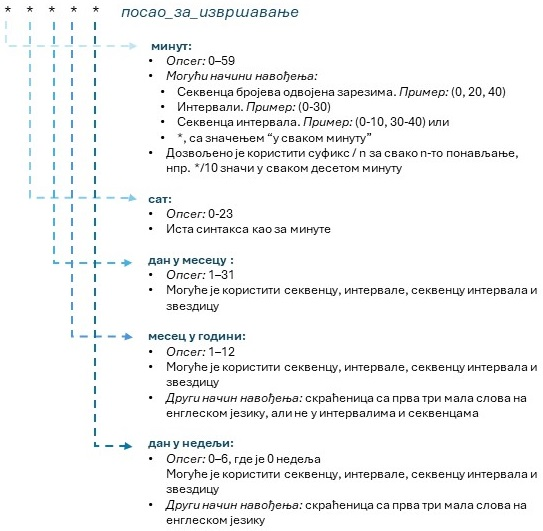
\includegraphics[scale=0.9]{assets/pictures/crontab_syntax.jpg}
  \caption{Синтакса конфигурационе датотеке \texttt{crontab}}
  \label{pic:crontab_syntax}
\end{figure}

На пример, следећи унос ће покренути скрипту \texttt{/home/user/script.sh} сваког дана у 2:30 ујутру:

\lstset{
  language=Python,
  basicstyle=\ttfamily,
  keywordstyle=\color{blue},
  frame=single
}
\begin{lstlisting}
    30 2 * * * /home/user/script.sh
\end{lstlisting}

У Django апликацијама \cite{django_crontab}, Cron задаци се додају у \texttt{settings.py} модул у оквиру \texttt{CRONJOBS} променљиве:

\lstset{
  language=C,
  basicstyle=\ttfamily,
  keywordstyle=\color{blue},
  showstringspaces=false
}
\begin{lstlisting}
    CRONJOBS = [
        ('0 0 * * *', 'scheduled_job'),
        ('0 4 * * *', 'django.core.management.call_command',
        ['django_menagement_command']),
    ]
\end{lstlisting}

где је \texttt{scheduled\_job} функција дефинисана у пројекту, a \\
\texttt{django\_menagement\_command} уграђена Django menagement команда (попут \\ 
\texttt{migrate}, \texttt{collectstatic}, ...) или прилагођена команда креирана од стране корисника.

Да би се дефинисани Cron задаци извршавали, потребно их је додати са командом:

\lstset{
  language=Python,
  basicstyle=\ttfamily,
  keywordstyle=\color{blue}
}
\begin{lstlisting}
    python manage.py crontab add
\end{lstlisting}

Додате задатке је могуће уклонити наредном командом:

\lstset{
  language=Python,
  basicstyle=\ttfamily,
  keywordstyle=\color{blue}
}
\begin{lstlisting}
    python manage.py crontab remove
\end{lstlisting}

У апликацији \textit{Train Wiser} се користе два Cron посла, један који на сваких сат времена уписује претходне активности корисника у базу и други за додавање детаља о новим активностима корисника.

\subsubsection{Мрежне куке}

\textit{Мрежне куке (енг. webhooks)} пружају начин за аутоматизацију комуникације између различитих сервиса путем HTTP захтева. Када се одређени догађај деси у изворном систему, HTTP захтев ће се аутоматски послати одредишном систему, најчешће садржећи корисне податке о догађају које одредишни систем захтева. Периодично слање захтева изворном систему ради провере да ли постоје нови или ажурирани догађаји (енг. \textit{pooling}) може бити неефикасно и оптеретити изворни систем. Коришћењем мрежних кука апликација ће добити информације о догађајима у реалном времену и искључиво онда када се догађаји десе. На тај начин се омогућава уштеда ресурса и ефикасна комуникација. 

Мрежне куке се јако често користе на \textit{SaaS (енг. software as a service)} платформама, будући да оне на основу активности које се дешавају подржавају креирање различитих типова догађаја. Да би апликација могла да добија HTTP захтеве мрежних кука, потребно је да се региструје за догађаје за које их изворна платформа нуди, као и да обезбеди веб адресу на коју ће се захтеви слати. \cite{webhooks_hookdeck, strava_webhooks}

% !# nema podrske za prelamanje engleskih reci
% тодо: проверити да ли је раније написано да се апп повезује са стравом
% todo: da li ovde naziv da bude povezivanje sa stravom?
\paragraph{Коришћење мрежних кука у апликацији \textit{Train Wiser}} Апликација \\ 
Strava подржава мрежне куке за одређене промене у личним подацима 
и активностима корисника, и охрабрује све API апликације да их користе. 

Када се догађај за који је мрежна кука везана догоди, POST захтев се шаље на веб адресу дефинисану од стране апликације. Очекивано је да апликација узврати одговор са статусом 200 у оквиру 2 секунде. Уколико се то не деси, POST захтев се понавља још максимално два пута, стога се саветује да се добијене информације обрађују асинхроно уколико је за обраду потебно више времена.

Да би се апликација регистровала за мрежне куке апликације Strava,
потребно је да се креира POST захтев ка адреси \url{https://www.strava.com/api/v3/push_subscriptions}. Очекивано је да захтев садржи параметре у URL формату који укључују клијетски идентификатор и клијентски тајни кључ апликације, тј. креденцијале апликације за приступ Strava ресурсима, поменуте у подпоглављу \ref{subsec:authorization_and_authentication}, затим, веб адресу повратног позива дефинисану од стране апликације на којој ће се захтеви слати \textit{(URL callback)} и јединствени токен дефинисан од стране власника апликације који ће апликација Strava узвратити слањем верификационог GET захтева ка адреси апликације. Верификациони GET захтев поред токена садржи и два поља чије вредности су ниске карактера, \textit{hub.mode} који је увек фиксне вредности \textit{''subscribe''}, и \textit{hub.challenge}, чија је вредност насумична ниска коју апликација узвраћа као одговор Strava апликацији затварајући процес креирања регистрације.  % можда доделити овој апп неки назив?  
\cite{strava_webhooks}

\colorbox{yellow}{Да ли додати како је одређена регистрација у \textit{Train Wiser} апликацији?}

Од догађаја за које се мрежне куке нуде од стране апликације Strava, за формирање скупа података са активностима вежбача за \textit{Train Wiser} апликацију је релевантно креирање нових активности.

Након што корисник постави нову активност и апликација \textit{Train Wiser} добије POST захтев мрежне куке, у базу у којој се чувају активности \\(\textit{StravaActivity}) ће се уписати идентификатор активности и идентификатор корисника који је додао активност. Дохватање детаљних информација о активности се ради коришћењем Django Cron посла који ће на сваких сат времена у тридесетом минуту проверити да ли у бази постоје активности које нису попуњене, тј. садрже само идентификатор активности и страни кључ ка StravaAthlete бази. 

\subsection{Формирање скупа података са резултатима трка}
\label{subsec:scrapy_desc}

Скуп података са резултатима трка је формиран на основу резултата са сајтова \href{https://www.runtrace.net}{runtrace.net}, \href{https://www.trka.rs}{trka.rs} и \href{https://www.bgdmarathon.org}{bgdmarathon.org} за које је добијена потврда да се јавно доступни подаци могу користити у истраживачке сврхе. Подаци са ових сајтова су обрађени \textit{техником кроловања (енг. crawling)} и \textit{екстракцијом података (енг. scraping)}.

Преузимање података од стране програма на било који други начин осим директном комуникацијом програма са API-ем странице представља технику екстракције података. Коришћење екстракције података уместо API-ја се саветује када % тодо: види да ли да остављаш апи
API није доступан или онда када јесте доступан, али формат података који пружа није одговарајући или постоји ограничење у обиму и учесталости захтева који се могу послати. Екстрактори веб података су ефикасан алат за прикупљање и обраду великих количина података са различитих веб страница. \cite{web_scraping_with_python} Кроловање података представља аутоматско извршавање програма за систематску претрагу веб страница и индексирање њиховог садржаја. Индексирање омогућава претраживачима да брзо и ефикасно пронађу релевантне информације у зависности од употребе. \cite{web_crawler}

Кроловање и екстракција података са веб страница у \textit{Train Wiser} апликацији су одрађени коришћењем оквира Scrapy. Scrapy је оквир отвореног кода програмског језика Python за веб кроловање и екстракцију структуираних података са HTML/XML страница. Често се користи за анализу и процесирање података, надгледање активности, аутоматизацију тестирања и историјско архивирање. Главна одлика овог алата је да захтеве распоређује и процесира асинхроно што му омогућава веома брзо кроловање у односу на секвенциони приступ будући да се више захтева може процесирати у исто време уз постојање толеранције грешака. 

Oвај оквир пружа једноставан API са доста могућности који је лако прилагодљив потребама програмера. Екстракција података се ради коришћењем проширених CSS селектора и XPath израза, док су JSON, CSV и XML формат на располагању на излазу. \cite{scrapy_doc} За потребе \textit{Train Wiser} апликације, екстрактовани подаци су експортовани у JSON формат. % тодо: опиши даље како извледа скуп и како си оформила јединствен јсон фајл

\section{Архитектура и дизајн апликације}

\colorbox{magenta}{(In progress)} За архитектуралну организацију апликације је одабран клијент-сервер модел. Клијентска апликација (енг. \textit{frontend}) је задужена за комуникацију са корисником и прослеђивање захтева серверској апликацији (енг. \textit{backend}) која је задужена за унутрашњу логику.

\section{Могућа унапређења}

\chapter{Коришћење апликације \textit{Train Wiser}}

\chapter{Имплементација модела машинског учења}
\section{Прикупљање података} % promeni u prilagodjavanje podataka

\colorbox{magenta}{(In progress)} Поступак формирања скупа података са резултатима трка описан је у подпоглављу \ref{subsec:scrapy_desc}. Број укупно сакупљених података са сајтова дат је у табелици \ref{tbl:rezultati_trka}:

\begin{table}[H]
\centering
\label{tbl:rezultati_trka}
\begin{tabular}{| >{\centering\arraybackslash} m{0.35\linewidth} | >{\centering\arraybackslash} m{0.35\linewidth} | >{\centering\arraybackslash} m{0.3\linewidth} |}
\hline
\textbf{Сајт} & \textbf{Укупан број резултата релевантних трка} & \textbf{? - ТОДО} \\
\hline
runtrace.net \rule{0pt}{1em} & 19708 & \\
\hline
trka.rs \rule{0pt}{1em} & 37491 & \\
\hline
bgdmarathon.org \rule{0pt}{1em} & 50275 & \\
\hline
\end{tabular}
\caption{Број података са сваког од сајта са резултатима трка}
\end{table}
 

\section{Евалуација модела}
\section{Могућа унапређења}

% ------------------------------------------------------------------------------


% ------------------------------------------------------------------------------
\chapter{Закључак}
ТОДО: Описати укратко шта је одрађено у раду и шта је закључак
% ------------------------------------------------------------------------------


% ------------------------------------------------------------------------------
% Literatura
% ------------------------------------------------------------------------------
\literatura

% ==============================================================================
% Završni deo teze i prilozi
\backmatter
% ==============================================================================

% ------------------------------------------------------------------------------
% Biografija kandidata
\begin{biografija}
\end{biografija}
% ------------------------------------------------------------------------------

\end{document} 